\section{Lösungen zum Abschnitt 2}

\begin{loes}\hypertarget{loes:2.1}
	Sei $a,b,c,d \in \R $.
	Dann erhalten wir durch
	\begin{align*}
	\begin{pmatrix}
	a & b \\
	c & d
	\end{pmatrix}
	\cdot
	\begin{pmatrix}
	1 & 0 \\
	0 & -1
	\end{pmatrix}
	&=
	\begin{pmatrix}
	a & -b \\
	c & -d
	\end{pmatrix} \\
	\begin{pmatrix}
	1 & 0 \\
	0 & -1
	\end{pmatrix}
	\cdot
	\begin{pmatrix}
	a & b \\
	c & d
	\end{pmatrix}
	&=
	\begin{pmatrix}
	a & b \\
	-c & -d
	\end{pmatrix},
	\end{align*}
	dass $ b = c = 0 $ gelten muss. Da unsere Matrix in $ \Gl_2(\R) $ enthalten sein muss, sollte dann $ a, d \neq 0 $ gelten. Also erhalten wir 
	\begin{align*}
	C_{\Gl_2(\R)}(S) := \lbrace \begin{pmatrix}
	a & 0 \\
	0 & d
	\end{pmatrix} \ | \ a,d \neq 0 \rbrace
	\end{align*}
	als Zentralisator. In diesem befinden sich alle invertierbaren Diagonalmatrizen und das Produkt von Diagonalmatrizen ist wieder eine Diagonalmatrix.
	Also ist unser Zentralisator eine Untergruppe. Dieser ist jedoch kein Normalteiler, denn für 
	$ a \neq b $ gilt
	\begin{align*}
	\begin{pmatrix}
	1 & 1 \\
	0 & 1
	\end{pmatrix}
	\cdot
	\begin{pmatrix}
	a & 0 \\
	0 & b
	\end{pmatrix}
	&= 
	\begin{pmatrix}
	a & b \\
	0 & b
	\end{pmatrix}
	\\
	\begin{pmatrix}
	a & 0 \\
	0 & b
	\end{pmatrix}
	\cdot
	\begin{pmatrix}
	1 & 1 \\
	0 & 1
	\end{pmatrix}
	&= 
	\begin{pmatrix}
	a & a \\
	0 & b
	\end{pmatrix}.
	\end{align*}
\end{loes}

\begin{loes}\hypertarget{loes:2.2}
	\
	\begin{enumerate}
		\item[a)]
		Für die Lösung dieser Aufgabe betrachten wir zunächst ein Bild.
		\begin{figure}[H]
			\centering
			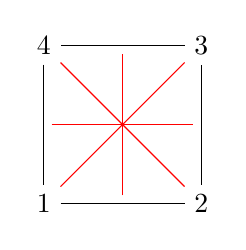
\begin{tikzpicture}
			\node (A) at (-1,-1)  {$1$};
			\node (B) at (1,-1) {$2$};
			\node (C) at (1,1) {$3$};
			\node (D) at (-1,1) {$4$};
			
			
			%\node (X) at (-0.5,0.69) {$ a $};
			%\node (Y) at (-0.7,0.19) {$ b $};
			%\node (Z) at (-0.7,-0.50) {$ c $};
			
			\draw[-] (A) to (B);
			\draw[-] (B) to (C);
			\draw[-] (C) to (D);
			\draw[-] (D) to (A);
			
			\draw[-,red] (-0.9,0) to (0.9,0);
			\draw[-,red] (A) to (C);
			\draw[-,red] (B) to (D);
			\draw[-,red] (0,-0.9) to (0,0.9);
			\end{tikzpicture}
		\end{figure}
		Mit einem Quadrat können wir vier Rotationen um $ 90^\circ $ ausführen und kommen dann an der Ausgangsstellung.
		Weiter können wir das Quadrat an den rot eingezeichneten Achsen spiegeln.
		Damit ergeben sich für die Rotationen 
		\begin{align*}
		r  &= (1234) \\
		r^2 &= (13)(24) \\
		r^3 &= (1432) \\
		r^4 &= \id
		\end{align*}
		und für die Spiegelungen
		\begin{align*}
		s_1 &= (14)(23) =: s\\
		s_2 &= (24)		= sr\\
		s_3 &= (12)(34)  = sr^2\\
		s_4 &= (13)		= sr^3.
		\end{align*}
		Damit haben wir alle Möglichkeiten aufgeführt.
		Wir bezeichnen diese Gruppe als \bi{Diedergruppe} vierten Grades und schreiben hierfür $ D_4 $.
		\index{Diedergruppe}
		Für diese gilt $ |D_4 | = 2 \cdot 4 = 8 $.
		
		\item[b)] 
		Nun interessieren wir uns für das Zentrum von $ G $.
		Ohne Zweifel gilt $ \id \in Z(G) $. Durch Ausprobieren erhalten wir noch
		$ (13)(24) \in Z(G) $.
		Dies lässt sich leicht mit Bildern verdeutlichen.
		
		\item[c)] 
		Wir wissen, dass $ |D_4 | = 8  $ gilt. Also erhalten wir mit dem Satz von Lagrange
		$ 1 ,2 ,3 $ und $ 8 $ als mögliche Untergruppenordnungen.
		Diese arbeiten wir nun nacheinander ab.
		Für die Ordnung $ 1 $ ist $ \lbrace \id \rbrace \leq D_4 $.
		Die zyklischen Untergruppen der Ordnung $ 2 $ sind
		\begin{align*}
		\langle (13) \rangle ,\langle(23) \rangle, \langle (13)(24) \rangle, \langle (12)(34) \rangle,
		\langle (14)(23) \rangle.
		\end{align*}
		und durch 
		\begin{align*}
		\langle (1234) \rangle &= \langle (1432) \rangle\\
		\langle (12)(34),(13)(24) \rangle &= \langle (14)(23), (13)(24) \rangle\\
		\langle (13),(24) \rangle &
		\end{align*}
		erhalten wir die Untergruppen der Ordnung 4.
		Mit
		\begin{figure}[H]
			\centering
			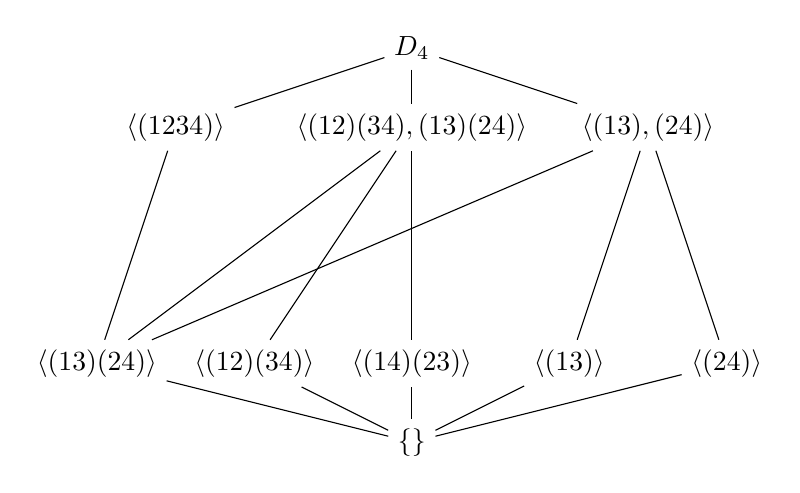
\begin{tikzpicture}
			\node (A) at (0,0)  {$\lbrace \id \rbrace$};
			
			\node (B) at (-4,1) {$\langle (13)(24) \rangle$};
			\node (C) at (-2,1) {$\langle (12)(34) \rangle$};
			\node (D) at (0,1) {$\langle (14)(23) \rangle$};
			\node (E) at (2,1) {$\langle (13) \rangle$};
			\node (F) at (4,1) {$\langle (24) \rangle$};
			
			\node (G) at (-3,4) {$\langle (1234) \rangle$};
			\node (H) at (0,4) {$\langle (12)(34),(13)(24) \rangle$};
			\node (I) at (3,4) {$\langle (13),(24) \rangle$};
			
			\node (J) at (0,5) {$D_4$};
			
			\draw[-] (A) to (B);
			\draw[-] (A) to (C);
			\draw[-] (A) to (D);
			\draw[-] (A) to (E);
			\draw[-] (A) to (F);
			
			\draw[-] (B) to (G);
			\draw[-] (B) to (H);
			\draw[-] (B) to (I);
			
			\draw[-] (C) to (H);
			\draw[-] (D) to (H);
			
			\draw[-] (E) to (I);
			\draw[-] (F) to (I);
			
			\draw[-] (J) to (G);
			\draw[-] (J) to (H);
			\draw[-] (J) to (I);
			\end{tikzpicture}
		\end{figure}
		sollen die Teilmengenbeziehungen dargestellt werden. Das Diagramm ist von unten nach oben zu lesen.
	\end{enumerate}
\end{loes}

\begin{loes}\hypertarget{loes:2.3}
	Sei $ H \leq G = \langle g \rangle $. Falls $ H  $ die triviale Untergruppe ist haben wir nichts zu zeigen.
	Sei also $ H \neq \lbrace e \rbrace $.
	Dann enthält $ H $ ein Element mit $ g^l \neq e , \ l \in \Z$. Dann gilt aufgrund der Untergruppeneigenschaft
	$ g^{-l} \in H $.
	Aus diesem Grund nehmen wir an, dass $ l > 0  $ ist und wir setzen
	$ k := \min \lbrace l > 0 \ | \ g^l \in H \rbrace $.
	Wir wollen nun zeigen, dass $ H = \langle g^k \rangle $ gilt.
	Sei $ a = g^j $ ein beliebiges Element aus $ G $. 
	Durch Division mit Rest gilt
	\begin{align*}
	j = q \cdot k + r
	\end{align*}
	für $ 1 \leq r < k $.
	Ist nun $ a \in H $, so muss aufgrund der Untergruppeneigenschaft
	\begin{align*}
	g^r = (g^k)^{-q} \cdot a \in H
	\end{align*}
	gelten. Aus der Minimalität folgt dann $ r = 0 $.
\end{loes}

\begin{loes}\hypertarget{loes:2.4}\
	\begin{enumerate}
		\item[a)]
		Sei $ h \in G $ beliebig, aber fest.
		Mit
		\begin{align*}
		\gamma_h(g_1 g_2) = h^{-1} g_1 g_2 h 
		=h^{-1} g_1 h h^{-1} g_2 h = \gamma_h(g_1) \cdot \gamma_h(g_2) 
		\end{align*}
		für alle $ g_1,g_2 \in G $ erhalten wir die Homomorphismuseigenschaft für $ \gamma_h $.
		Durch schnelles Nachrechnen erhalten wir als Umkehrabbildung $ \gamma_{h^{-1} }$.
		Damit ist $ \gamma_h $ bijektiv.
		
		\item[b)]
		Sei $ \operatorname{Inn}(G) $ die Menge der inneren Automorphismen.
		Nun sei $ \varphi \in \Aut(G) $ und $ g,h \in G $ beliebig.
		Dann folgt mit
		\begin{align*}
		(\varphi \circ \gamma_h \circ \varphi^{-1})(g)
		= \varphi \circ \gamma_h(\varphi^{-1}(g))
		= \varphi(h^{-1} \varphi^{-1}(g) h)
		= \varphi(h)^{-1} \cdot g \cdot \varphi(h)
		= \gamma_{\varphi(h)}(g),
		\end{align*}
		dass $ \operatorname{Inn}(G) \nt \Aut(G) $ gilt.
		Die Untergruppeneigenschaften stehen nach dem Aufschreiben sofort da.
		
	\end{enumerate}
\end{loes}

\begin{loes}\hypertarget{loes:2.5}\
	\begin{enumerate}
		\item[a)]
		Es gilt
		\begin{align*}
		N_G(H) = \lbrace g \in G \ | \ g^{-1} H g = H \rbrace
		\end{align*}
		und mit $ H \nt K $ folgt sofort $ H \subset N_G(H) $.
		
		\item[b)]
		Zuerst müssen wir zeigen, dass $ K \cdot H \leq G $ gilt.
		Zunächst gilt $ K \leq N_G(H) $, das heißt
		\begin{align*}
		k^{-1} H k = H
		\end{align*}
		für alle $ k \in K $.
		Nun wenden wir das Untergruppenkriterium an.
		Seien $ k_1 , k_2  \in K$ und $ h_1, h_2 \in H $ beliebig.
		Dann folgt mit
		\begin{align*}
		k_1 h_1(k_2 h_2)^{-1}
		= k_1 h_1 h_2^{-1} k_2^{-1}
		= k_1 h_1 k_2^{-1}\underbrace{k_2 h_2^{-1} k_2^{-1}}_{=: \tilde{h}}
		= \underbrace{k_1 k_2^{-1}}_{\in K } \underbrace{k_2 h_1 k_2^{-1} \tilde{h}}_{\in H} \in K \cdot H
		\end{align*}
		die Untergruppeneigenschaft.
		Nun fehlt noch $ H \nt K \cdot H $.
		Dies erhalten wir durch
		\begin{align*}
		(kh)^{-1} H kh
		= h^{-1} k^{-1} H k h
		= H
		\end{align*}
		für $ k \in K  $ und $ h \in H  $ sofort.
	\end{enumerate}
\end{loes}

\begin{loes}\hypertarget{loes:2.6}\
	\begin{enumerate}
		\item[a)]
		Wir müssen zwei Fälle betrachten.
		Sei zunächst $ v = 0 $.
		Dann gilt $ A \cdot v = 0  $ für alle $ A \in \Sl_n(\R) $
		und folgt $ v \in O_0 $.
		Nun betrachten wir $ v \neq 0  $ und ergänzen $ v $ mithilfe 
		des Basisergänzungssatz zu einer Basis von $ \R^n $.
		Diese sei $ \lbrace v , b_2 , \dots , b_n  \rbrace$ und mit
		\begin{align*}
		M := \begin{pmatrix}
		v & b_2 & \hdots & b_n
		\end{pmatrix}
		\end{align*}
		erhalten wir eine invertierbare Matrix mit $ M \cdot e_1 = v $ und $ \det(M) \neq 0 $.
		Mit 
		\begin{align*}
		\tilde{M} = \begin{pmatrix}
		v & \frac{1}{\det(M)} \cdot b_2 & \hdots & b_n
		\end{pmatrix}
		\end{align*}
		gilt noch $ \tilde{M} \in \Sl_n(\R) $, womit $ v \in O_{e_1} $ folgt.
		Insgesamt gibt es also die zwei Bahnen $ O_0 $ und $ O_{e_1} $.
		
		\item[b)] 
		Der Fall, dass $ v = 0 $ ist, sollte nach a) klar sein.
		Nun betrachten wir $ || v || =  \lambda $ mit $ \lambda > 0 $.
		Mit dem Basisergänzungssatz und Gram-Schmidt-Verfahren erhalten wir eine ONB.
		In $ A $ seien die Spalten dieser ONB.
		Dann gilt 
		\begin{align*}
		A \cdot e_1 = \frac{1}{\lambda} \cdot v
		\Leftrightarrow
		A \cdot (\lambda e_1) = v
		\end{align*}
		und wir erhalten mit
		\begin{align*}
		\R^n = O_0 \cup \bigcup \limits_{\lambda > 0} O_{\lambda e_1}
		\end{align*}
		alle Bahnen.
		
		\item[c)]
		Wir betrachten 
		\begin{align*}
		\begin{pmatrix}
		\lambda_1 & \hdots & 0\\
		\vdots  &\ddots & \vdots \\
		0  & \hdots & \lambda_n
		\end{pmatrix}
		\cdot
		\begin{pmatrix}
		\bullet \\
		\vdots \\
		\bullet
		\end{pmatrix}
		= 
		\begin{pmatrix}
		\lambda_1\cdot \bullet \\
		\vdots \\
		 \lambda_n \cdot\bullet
		\end{pmatrix}
		\end{align*}
		und erkennen, dass es nur relevant ist, welche Punkte ungleich null sind.
		Zur Vereinfachung vereinbaren wir, dass die Punkte nur die Werte $ 0 $ oder $ 1 $
		annehmen können.
		Dadurch erhalten wir ein kombinatorisches Problem.
		Durch 
		\begin{align*}
		\sum \limits_{k=0}^n \binom{n}{k}
		=
		\sum \limits_{k=0}^n \binom{n}{k} \cdot 1^{n-k} \cdot 1^k
		=2^n
		\end{align*}
		erhalten wir die Anzahl der möglichen Bahnen.
		
		\item[d)]
		Für $ v = 0  $ erhalten wir wieder eine Bahn.
		Nun gilt für eine invertierbare oberer Dreiecksmatrix $ A $ und 
		$ 1 \leq k \leq n $
		\begin{align*}
		A \cdot e_k = 
		\begin{pmatrix}
		a_{k1}\\
		\vdots\\
		a_{k(k-1)}\\
		a_{kk}
		\end{pmatrix}
		\end{align*}
		mit $ a_{kk} \neq 0 $.
		Damit erhalten wir mit
		\begin{align*}
		O_{e_1} &= \left\lbrace 
		\begin{pmatrix}
		x_1 \\
		0\\
		\vdots\\
		0	
		\end{pmatrix}
		\ | \ x_1 \in \R \wedge x_1 \neq 0 \right\rbrace \\
		&\vdots\\
		O_{e_n} &= \left\lbrace 
		\begin{pmatrix}
		x_1 \\
		x_2\\
		\vdots\\
		x_n	
		\end{pmatrix}
		\ | \ x_1,\dots ,x_n \in \R \wedge x_n \neq 0 \right\rbrace 
		\end{align*}
		alle Bahnen.
	\end{enumerate}
\end{loes}

\begin{loes}\hypertarget{loes:2.7}\
	\begin{enumerate}
		\item[a)]
		 Sei $ G $ eine Gruppe mit zwei disjunkten Konjugationsklassen.
		 Dann muss
		 \begin{align*}
		 G = \lbrace e \rbrace \cup \lbrace h^{-1} g h \ | \ h \in G \rbrace
		 \end{align*}
		 für $ g \in G \setminus \lbrace e \rbrace $ gelten.
		 Mit der Klassengleichung erhalten wir:
		 \begin{align*}
		 n := |G| = \frac{|G|}{|C_G(e)|} + \frac{|G|}{|C_G(g)|}
		 = 1 + \frac{|G|}{|C_G(g)|}
		 \Leftrightarrow
		 n-1 = \frac{|G|}{|C_G(g)|}
		 \Leftrightarrow
		 |C_G(g)| = \frac{n}{n-1} \in \N
		 \end{align*}
		 Damit kommt für $ n $ nur die $ 2 $ infrage, womit $ G \cong C_2 $ gilt.
		 
		 \item[b)]
		 Sei $ G $ eine $ p$- Gruppe mit drei disjunkten Konjugationsklassen.
		 Dann gilt
		 \begin{align*}
		 | G | &= | C_e | + | C_2 | + | C_3 |\\
		 \Leftrightarrow
		 p^k &= 1 + p^l + p^m
		 \end{align*}
		 mit $ l, m < k $.
		 Falls $ l = 0  $ und $ r = 0 $ ist, gilt
		 \begin{align*}
		 |G| = 3 \Rightarrow G \cong C_3.
		 \end{align*}
		 Gilt $ l = 0  $ und $ m \neq 0 $, so folgt
		 \begin{align*}
		 p^k = 2 + p^m
		 \Rightarrow p^m \mid p^k \wedge 2 \mid p^k
		 \Rightarrow p^2
		 \end{align*}
		 und mit 
		 \begin{align*}
		 p^k - p^m = 2 
		 \Leftrightarrow
		 1 = 2^{m-1} \cdot (2^{k-m} - 1 ) 
		 \end{align*}
		 folgt weiter, dass $ m = 1$ und $ k = 2 $ sein muss.
		 Mit Aufgabe 4 auf Blatt 3 ist $ G $ somit abelsch.
		 Damit besitzt $ G $ vier Konjugationsklassen.
		 Dies ist ein Widerspruch.
		 Nun fehlt noch $ l \neq 0 $ und $ m \neq 0 $.
		 Hier folgt direkt mit
		 \begin{align*}
		 p^k = 1 + p^l + p^m
		 \Leftrightarrow 
		 p^k - p^l - p^m  = 1
		 \Rightarrow 
		 p \mid 1
		 \end{align*}
		 ein Widerspruch.
	\end{enumerate}
\end{loes}

\begin{loes}\hypertarget{loes:2.8}\
	\begin{enumerate}
		\item[a)]
		Wir nehmen an der Index von $ Z(G) $ ist gleich $ p $.
		Nun folgt mit dem guten alten Lagrange, dass die
		Faktorgruppe $ | G/Z(G) | = p  $ zyklisch ist.
		Damit ist diese auch abelsch
		und es folgt $ G = Z(G) $.
		Aber dann müsste der Index von $ Z(G) $ gleich $ 1 $ sein.
		Somit war unsere Annahme falsch.
		
		\item[b)]
		Nach Lagrange muss $ |Z(G) |  $ teilt $ | G| $ gelten.
		Damit haben wir $ 1 $, $ p $ oder $ p^2 $ als Möglichkeiten.
		Nach  \ref{skript:2.10}  fällt die erste davon raus.
		Die zweite geht aufgrund der a) nicht.
		Für die dritte folgt $ Z(G) = G $, womit $ G $ abelsch ist. 
	\end{enumerate}
\end{loes}

\begin{loes}\hypertarget{loes:2.9}\
	\begin{enumerate}
		\item[a)]
		Es folgt direkt, dass $ \id.x = x $ für alle $ x \in X $ gilt.
		Seien nun $ \sigma, \tau \in S_5 $ und $ x =(y_1,y_2) $ beliebig.
		Dann gilt
		\begin{align*}
		\sigma.(\tau.(y_1, y_2))
		= \sigma.(\tau(y_1),\tau(y_2)
		= (\sigma \circ \tau(y_1),\sigma \circ \tau(y_2))
		=(\omega \circ \tau).(y_1,y_2),
		\end{align*} 
		womit dies eine Gruppenoperation von $ G $ auf $ X $ ist.
		
		\item[b)]
		Wir wollen zeigen, dass es zwei Bahnen gibt.
		Sei $ i \in Y $ beliebig.
		Für alle $ j \in Y $ existiert mindestens ein $ \sigma \in S_5 $ 
		mit $ \sigma(i) = j $.
		Da Permutationen bijektiv sind, folgt
		\begin{align*}
		i \neq j &\Rightarrow \sigma(i) \neq \sigma(j)\\
		i = j &\Rightarrow \sigma(i) = \sigma(j)
		\end{align*}  
		für alle $ \sigma \in S_5 $.
		Damit sind 
		\begin{align*}
		O_{(1,1)} &= \lbrace (i,i) \ | \ i \in Y \rbrace\\
		O_{(1,2)} &= \lbrace (i,j) \ | \ i,j \in Y \wedge i \neq j\rbrace
		\end{align*}
		die gesuchten Bahnen.
		
		\item[c)]
		Für $ x_1 =(5,5) $ und $ x_2 = (4,5) $ gelten
		\begin{align*}
		\Stab_G(x_1) \cong S_4 \quad 
		\Stab_G(x_2) \cong S_3.
		\end{align*}
		Dies steht direkt nach dem Aufschreiben da.
		Wer lustig drauf ist, kann sich natürlich die Isomorphismen aufschreiben.
		Der gesuchte Zusammenhang ist 
		\begin{align*}
		|O_x| = \frac{|G|}{|\Stab_G(x)|}
		\end{align*}
		für $ x \in X $.
		Damit ergeben sich auch
		\begin{align*}
		|O_{(1,1)}| = 5 \quad \wedge \quad |O_{(1,2)}| = 25,
		\end{align*}
		was uns die Existenz von zwei Bahnen nochmal bestätigt.
	\end{enumerate}
\end{loes}